\chapter{HASIL DAN PEMBAHASAN}
\label{chap:hasildanpembahasan}

% Ubah bagian-bagian berikut dengan isi dari pengujian dan analisis

Pada penelitian ini dipaparkan hasil penelitian beserta analisis dari model re-identifikasi yang telah dibuat sesuai dengan 
yang telah dijelaskan di Bab 3. Model re-identifikasi yang telah dibuat akan diuji cobakan menggunakan data test dari dataset 
VRIC yang telah disiapkan. 

\section{Hasil Penelitian}
\label{sec:hasilpenelitian}

Pada penelitian ini, telah ditentukan 4 jenis model re-identifikasi yang berbeda berdasarkan jenis model dan pengaturan 
hyper-parameternya. Dan pada setiap jenis model, dilakukan 3 iterasi re-identifikasi untuk menentukan model re-identifikasi 
terbaik di setiap jenisnya. Sehingga total model yang diciptakan pada penelitian ini berjumlah 12 model. 

Dalam proses \emph{deep learning} khususnya pada tahap \emph{training} dan \emph{validation}, terdapat nilai yang dapat 
menunjukan bagus atau tidaknya model yang telah diciptakan. Nilai tersebut adalah nilai loss dan nilai top 1 error, yang 
dapat menunjukan performa dari sebuah model saat tahapan \emph{training} dan \emph{validation} berlangsung. Dengan total 
epoch sebesar 60 untuk setiap model, akan didapatkan model dengan nilai loss dan nilai top 1 error terendah. 

\subsection{Swin Transformer V1 Parameter 1}

Pada Swin Transformer V1 parameter 1, hyper-parameter yang ditentukan yaitu sebagai berikut:

\begin{itemize}[nolistsep]
  \item Epoch = 60
  \item Batch Size = 32
  \item Random Erasing Probability = 0
  \item Learning Rate = 0.05
  \item Warm Epoch = 0
\end{itemize}

% Hasil nilai loss dan top 1 error pada Swin Transformer V1 dengan parameter 1 dapat dilihat pada gambar 
% 4.1, gambar 4.2, dan gambar 4.3.

\begin{figure}[ht]
  \centering
  % Nama dari file gambar yang diinputkan
  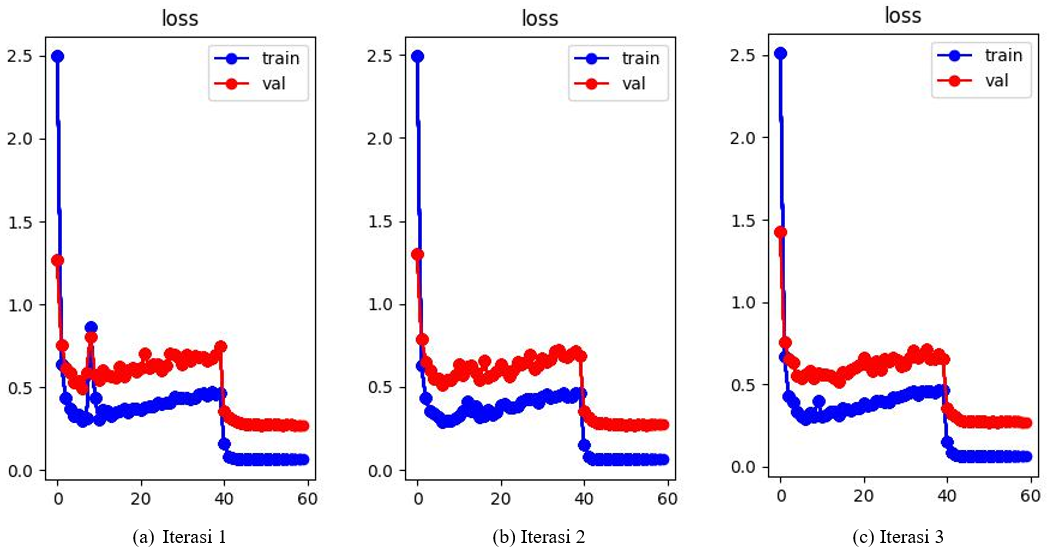
\includegraphics[scale=0.55]{gambar/Train SwinV1 Loss.png}
  % Keterangan gambar yang diinputkan
  \caption{Grafik Loss dari Masing-Masing Iterasi Swin Transformer V1 Parameter 1}
  % Label referensi dari gambar yang diinputkan
  \label{fig:grafiklossdantop1errdariswinv1parameter1iterasi1}
\end{figure}

\begin{figure}[ht]
  \centering
  % Nama dari file gambar yang diinputkan
  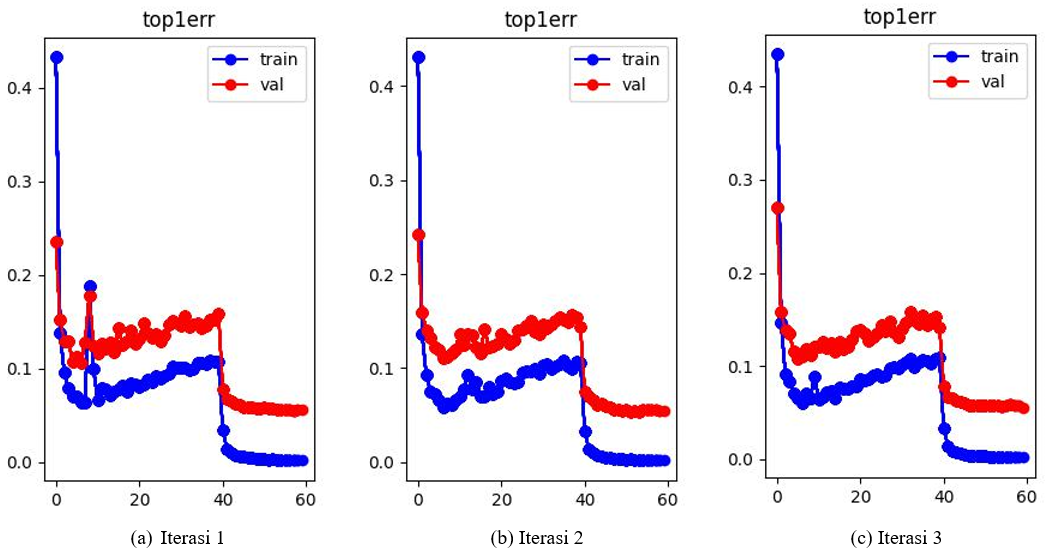
\includegraphics[scale=0.55]{gambar/Train SwinV1 Top1Err.png}
  % Keterangan gambar yang diinputkan
  \caption{Grafik Top 1 Error dari Masing-Masing Swin Transformer V1 Parameter 1}
  % Label referensi dari gambar yang diinputkan
  \label{fig:grafiklossdantop1errdariswinv1parameter1iterasi2}
\end{figure}

% \begin{figure}[ht]
%   \centering
%   % Nama dari file gambar yang diinputkan
%   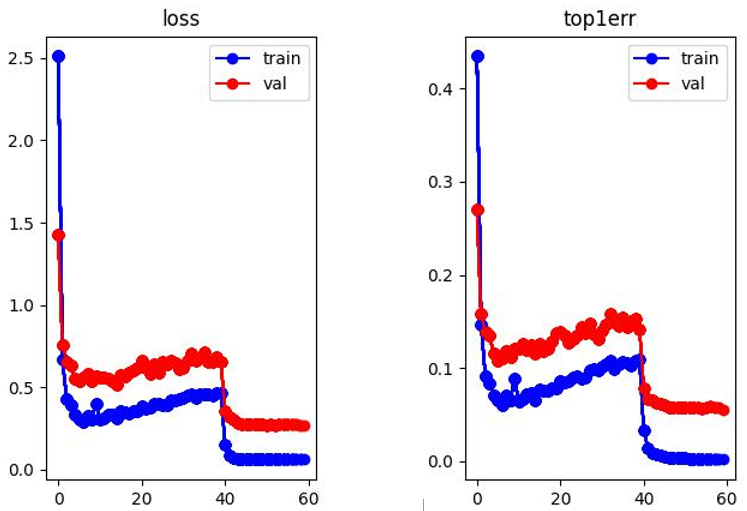
\includegraphics[scale=0.6]{gambar/Train SwinV1_2.png}
%   % Keterangan gambar yang diinputkan
%   \caption{Grafik Loss dan Top 1 Error dari Swin Transformer V1 Parameter 1 Iterasi 3}
%   % Label referensi dari gambar yang diinputkan
%   \label{fig:grafiklossdantop1errdariswinv1parameter1iterasi3}
% \end{figure}

Selain gambar grafik diatas, diperoleh pula nilai mAP, rank@1, rank@5, rank@10 dari proses 
\emph{Testing} pada masing-masing iterasi. Dari tiga kali iterasi tersebut, maka didapatkan 
rata-rata dari model Swin Transformer V1 Parameter 1. Seluruh nilai iterasi dan rata-ratanya 
dapat dilihat pada tabel 4.1.
% Diperoleh pula nilai mAP, rank@1, rank@5, rank@10 dari proses \emph{Testing} pada 
% masing-masing iterasi. Seluruh nilai tersebut dapat dilihat di tabel 4.2.

\begin{table}[h!]
  \begin{center}
  \caption{Nilai mAP, Rank@1, Rank@5, dan Rank@10 Swin Transformer V1 Parameter 1}
  \label{tb:NilaimAP,Rank1,Rank5,danRank10ModelSwinTransformerV1Parameter1}
  \begin{tabular}{|l|l|l|l|l|}
      \hline
      \textit{ } & \begin{tabular}[c]{@{}l@{}}\textbf{mAP}\end{tabular} & \begin{tabular}[c]{@{}l@{}}\textbf{Rank@1}\end{tabular} & \begin{tabular}[c]{@{}l@{}}\textbf{Rank@5}\end{tabular} & \begin{tabular}[c]{@{}l@{}}\textbf{Rank@10}\end{tabular}\\ \hline
      \textit{\textbf{Iterasi 1}} & \begin{tabular}[c]{@{}l@{}}0.667091\end{tabular} & \begin{tabular}[c]{@{}l@{}}0.622199\end{tabular} & \begin{tabular}[c]{@{}l@{}}0.820704\end{tabular} & \begin{tabular}[c]{@{}l@{}}0.870153\end{tabular}\\ \hline
      \textit{\textbf{Iterasi 2}} & \begin{tabular}[c]{@{}l@{}}0.667997\end{tabular} & \begin{tabular}[c]{@{}l@{}}0.621487\end{tabular} & \begin{tabular}[c]{@{}l@{}}0.827819\end{tabular} & \begin{tabular}[c]{@{}l@{}}0.869086\end{tabular}\\ \hline
      \textit{\textbf{Iterasi 3}} & \begin{tabular}[c]{@{}l@{}}\textbf{0.670210}\end{tabular} & \begin{tabular}[c]{@{}l@{}}\textbf{0.623621}\end{tabular} & \begin{tabular}[c]{@{}l@{}}\textbf{0.829598}\end{tabular} & \begin{tabular}[c]{@{}l@{}}\textbf{0.872643}\end{tabular}\\ \hline
      \textit{\textbf{Rata-Rata}} & \begin{tabular}[c]{@{}l@{}}0.668432\end{tabular} & \begin{tabular}[c]{@{}l@{}}0.622435\end{tabular} & \begin{tabular}[c]{@{}l@{}}0.826040\end{tabular} & \begin{tabular}[c]{@{}l@{}}0.870627\end{tabular}\\ \hline
  \end{tabular}
  \end{center}
\end{table}

\subsection{Swin Transformer V2 Parameter 1}

Pada Swin Transformer V2 parameter 1, hyper-parameter yang ditentukan yaitu sebagai berikut:

\begin{itemize}[nolistsep]
  \item Epoch = 60
  \item Batch Size = 32
  \item Random Erasing Probability = 0
  \item Learning Rate = 0.05
  \item Warm Epoch = 0
\end{itemize}

Dengan melakukan tiga kali iterasi menggunakan hyper-parameter yang disebutkan diatas, maka didapatkan hasil berupa grafik 
nilai loss dan top 1 error dari proses \emph{training} dan \emph{validation} untuk model Swin Transformer V2 
parameter 1 yang dapat dilihat pada gambar 4.3, dan gambar 4.4. Tiga kali iterasi dilakukan untuk mendapatkan 
hasil terbaik dari model Swin Transformer V2 parameter 1. \\
\\
\\

\begin{figure}[ht]
  \centering
  % Nama dari file gambar yang diinputkan
  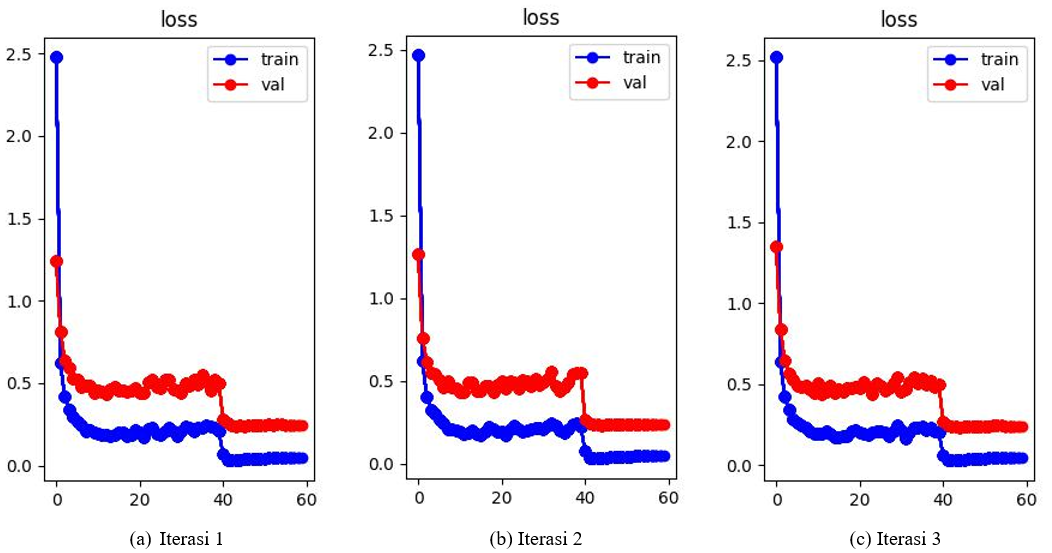
\includegraphics[scale=0.55]{gambar/Train SwinV2 Loss.png}
  % Keterangan gambar yang diinputkan
  \caption{Grafik Loss dari Masing-Masing Swin Transformer V2 Parameter 1}
  % Label referensi dari gambar yang diinputkan
  \label{fig:grafiklossdantop1errdariprosestrainingdanvalidationswinv2iterasi1}
\end{figure}

\begin{figure}[ht]
  \centering
  % Nama dari file gambar yang diinputkan
  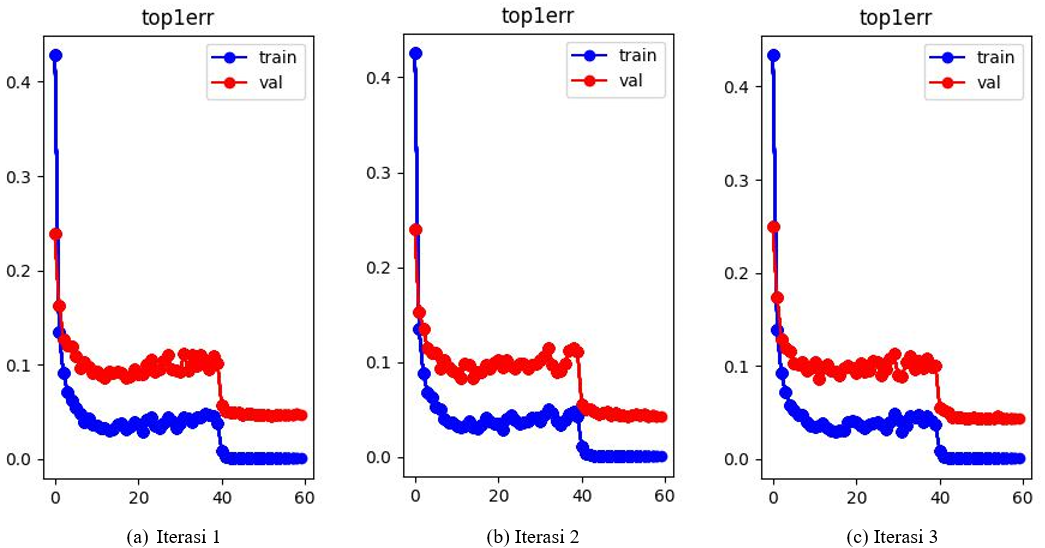
\includegraphics[scale=0.55]{gambar/Train SwinV2 Top1Err.png}
  % Keterangan gambar yang diinputkan
  \caption{Grafik Top 1 Error dari Masing-Masing Swin Transformer V2 Parameter 1}
  % Label referensi dari gambar yang diinputkan
  \label{fig:grafiklossdantop1errdariprosestrainingdanvalidationswinv2iterasi2}
\end{figure}

% \begin{figure}[ht]
%   \centering
%   % Nama dari file gambar yang diinputkan
%   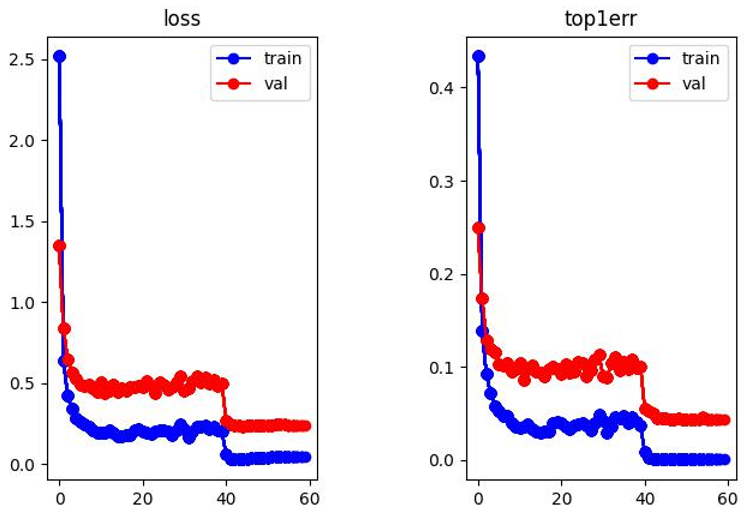
\includegraphics[scale=0.6]{gambar/Train SwinV2_2.png}
%   % Keterangan gambar yang diinputkan
%   \caption{Grafik Loss dan Top 1 Error dari Swin Transformer V2 Parameter 1 Iterasi 3}
%   % Label referensi dari gambar yang diinputkan
%   \label{fig:grafiklossdantop1errdariprosestrainingdanvalidationswinv2iterasi3}
% \end{figure}

Diperoleh pula nilai mAP, rank@1, rank@5, rank@10 dari proses \emph{Testing} pada 
masing-masing iterasi. Seluruh nilai tersebut dapat dilihat di tabel 4.2.

\begin{table}[h!]
  \begin{center}
  \caption{Nilai mAP, Rank@1, Rank@5, dan Rank@10 Swin Transformer V2 Parameter 1}
  \label{tb:NilaimAP,Rank1,Rank5,danRank10ModelSwinTransformerV1Parameter1}
  \begin{tabular}{|l|l|l|l|l|}
      \hline
      \textit{ } & \begin{tabular}[c]{@{}l@{}}\textbf{mAP}\end{tabular} & \begin{tabular}[c]{@{}l@{}}\textbf{Rank@1}\end{tabular} & \begin{tabular}[c]{@{}l@{}}\textbf{Rank@5}\end{tabular} & \begin{tabular}[c]{@{}l@{}}\textbf{Rank@10}\end{tabular}\\ \hline
      \textit{\textbf{Iterasi 1}} & \begin{tabular}[c]{@{}l@{}}\textbf{0.725377}\end{tabular} & \begin{tabular}[c]{@{}l@{}}\textbf{0.686233}\end{tabular} & \begin{tabular}[c]{@{}l@{}}0.857346\end{tabular} & \begin{tabular}[c]{@{}l@{}}0.895411\end{tabular}\\ \hline
      \textit{\textbf{Iterasi 2}} & \begin{tabular}[c]{@{}l@{}}0.719978\end{tabular} & \begin{tabular}[c]{@{}l@{}}0.678762\end{tabular} & \begin{tabular}[c]{@{}l@{}}\textbf{0.863750}\end{tabular} & \begin{tabular}[c]{@{}l@{}}\textbf{0.903949}\end{tabular}\\ \hline
      \textit{\textbf{Iterasi 3}} & \begin{tabular}[c]{@{}l@{}}0.715753\end{tabular} & \begin{tabular}[c]{@{}l@{}}0.674493\end{tabular} & \begin{tabular}[c]{@{}l@{}}0.854856\end{tabular} & \begin{tabular}[c]{@{}l@{}}0.897901\end{tabular}\\ \hline
      \textit{\textbf{Rata-Rata}} & \begin{tabular}[c]{@{}l@{}}0.720369\end{tabular} & \begin{tabular}[c]{@{}l@{}}0.679829\end{tabular} & \begin{tabular}[c]{@{}l@{}}0.858651\end{tabular} & \begin{tabular}[c]{@{}l@{}}0.899087\end{tabular}\\ \hline
  \end{tabular}
  \end{center}
\end{table}

\subsection{Swin Transformer V1 Parameter 2}
\subsection{Swin Transformer V2 Parameter 2}

% Hasil nilai 
% loss dan top 1 error dari \emph{training} dan \emph{validation} pada setiap model Swin Transformer dapat dilihat pada 
% gambar 4.1 hingga gambar 4.12.

\section{Analisa Hasil}
\label{sec:analisahasil}

% Dari tabel 4.1, tabel 4.2, serta grafik loss dan top 1 error yang ditampilkan pada bagian 4.1.1 dan 4.1.2, dapat diteliti 
% hasil model terbaik dari proses \emph{training} dan \emph{validation}. Iterasi dari masing-masing jenis model akan 
% mengambil hasil epoch terbaik dari proses \emph{training} dan \emph{validation}, sehingga hasil yang digunakan belum 
% tentu merupakan epoch terakhir dari proses \emph{training} dan \emph{validation}. Penjelasan terkait hasil dari setiap 
% jenis model yaitu sebagai berikut.

Dari tabel 4.1, tabel 4.2, serta grafik loss dan top 1 error yang ditampilkan pada bagian 4.1.1 dan 4.1.2, dapat diteliti 
hasil model terbaik dari proses \emph{training} dan \emph{validation}. Setiap jenis model re-identifikasi mobil akan 
mengambil hasil iterasi terbaik dari proses \emph{training} dan \emph{validation}, sehingga hasil yang digunakan pada 
pengujian belum tentu merupakan iterasi terakhir dari proses \emph{training} dan \emph{validation}. Penjelasan terkait 
hasil dari setiap jenis model yaitu sebagai berikut.

\subsection{Swin Transformer V1 Parameter 1}

Pada model Swin Transformer V1 parameter 1, model yang digunakan yaitu Swin-B (\emph{Base}), yang merupakan bentuk 
dasar dari arsitektur Swin Transformer. Dari tiga kali iterasi yang dilakukan, didapatkan data bahwa rata-rata nilai 
mAP (\emph{Mean Average Precision}) untuk model Swin Transformer V1 parameter 1 sebesar 0,668 atau 66,8\%. Dan untuk 
rank@1, rank@5, dan rank@10 berturut-turut sebesar 62,2\%, 82,6\%, dan 87,1\%. 

Berdasarkan Tabel 4.1, iterasi ketiga menjadi iterasi dengan hasil terbaik untuk model Swin Transformer V1 parameter 1. 
Hal ini didasarkan pada nilai mAP yang didapat yaitu sebesar 0.67 atau 67\%. Nilai tersebut 0,2\% lebih besar dari 
mAP rata-rata. Selain itu rank@1 yang didapat sebesar 62,4\% atau 0,2\% lebih besar dari rank@1 rata-rata. Rank@5 sebesar 
82,9\% atau 0,4\% lebih besar dari rank@5 rata-rata. Dan rank@10 sebesar 87,3\% atau 0,2\% lebih besar dari rank@10 
rata-rata.

\subsection{Swin Transformer V2 Parameter 1}

Pada model Swin Transformer V2 parameter 1, model yang digunakan yaitu Swin-B (\emph{Base}), yang merupakan bentuk 
dasar dari arsitektur Swin Transformer V2. Dari tiga kali iterasi yang dilakukan, didapatkan data bahwa rata-rata nilai 
mAP (\emph{Mean Average Precision}) untuk model Swin Transformer V2 parameter 1 sebesar 0,72 atau 72\%. Dan untuk 
rank@1, rank@5, dan rank@10 berturut-turut sebesar 67,9\%, 85,8\%, dan 89,9\%. 

Berdasarkan Tabel 4.2, iterasi pertama menjadi iterasi dengan hasil terbaik untuk model Swin Transformer V2 parameter 1. 
Hal ini didasarkan pada nilai mAP yang didapat yaitu sebesar 0.725 atau 72,5\%. Nilai tersebut 0,5\% lebih besar dari 
mAP rata-rata. Selain itu rank@1 yang didapat sebesar 68,6\% atau 0,7\% lebih besar dari rank@1 rata-rata. Namun 
Rank@5 memiliki nilai sebesar 85,7\% atau 0,1\% lebih kecil dari rank@5 rata-rata. Dan rank@10 sebesar 89,5\% atau 0,4\% 
lebih kecil dari rank@10 rata-rata.

\section{Skenario Pengujian}
\label{sec:skenariopengujian}

Pengujian dilakukan pada setiap model re-identifikasi mobil dengan iterasi terbaik pada masing-masing modelnya. Setiap 
model memiliki iterasi terbaiknya masing-masing yang telah dijelaskan pada bagian 4.2.1 dan 4.2.2. Dari hasil \emph{training} 
dan \emph{validation}, maka model dapat dilakukan \emph{testing} menggunakan data \emph{test} yang telah tersedia dari 
dataset VRIC.

Pengujian dilakukan dengan cara memasukkan sebuah gambar kueri ke dalam model re-identifikasi mobil. Model yang sudah memiliki 
galeri berisi kumpulan gambar mobil kemudian akan mencari gambar dengan objek (mobil) yang memilik kemiripan dengan gambar 
kueri di galeri. Beberapa gambar yang memiliki kemiripan tertinggi dengan kueri kemudian akan dibuat list tingkat kemiripan 
gambar galeri berdasarkan gambar kueri. Berikut merupakan hasil pengujian model re-identifikasi mobil menggunakan beberapa 
gambar kueri.

\subsection{Swin Transformer V1 Parameter 1}

Model Swin Transformer V1 parameter 1 menggunakan iterasi ketiga sebagai model pengujian re-identifikasi mobil. Berikut 
merupakan hasil re-identifikasi mobil dari Swin Transformer V1 parameter 1.

\subsection{Swin Transformer V2 Parameter 1}

Model Swin Transformer V2 parameter 1 menggunakan iterasi pertama sebagai model pengujian re-identifikasi mobil. Berikut 
merupakan hasil re-identifikasi mobil dari Swin Transformer V2 parameter 1.

\section{Analisa Pengujian}
\label{sec:analisapengujian}

% Dari pengujian yang \lipsum[1]

% % Contoh pembuatan tabel
% \begin{longtable}{|c|c|c|}
%   \caption{Hasil Pengukuran Energi dan Kecepatan}
%   \label{tb:EnergiKecepatan}                                   \\
%   \hline
%   \rowcolor[HTML]{C0C0C0}
%   \textbf{Energi} & \textbf{Jarak Tempuh} & \textbf{Kecepatan} \\
%   \hline
%   10 J            & 1000 M                & 200 M/s            \\
%   20 J            & 2000 M                & 400 M/s            \\
%   30 J            & 4000 M                & 800 M/s            \\
%   40 J            & 8000 M                & 1600 M/s           \\
%   \hline
% \end{longtable}

% \lipsum[2-4]
